\documentclass[letterpaper]{article} % DO NOT CHANGE THIS
\usepackage{aaai2027}  % DO NOT CHANGE THIS
\usepackage[hyphens]{url}  % DO NOT CHANGE THIS
\usepackage{graphicx} % DO NOT CHANGE THIS
\urlstyle{rm} % DO NOT CHANGE THIS
\def\UrlFont{\rm}  % DO NOT CHANGE THIS
\usepackage{natbib}  % DO NOT CHANGE THIS AND DO NOT ADD ANY OPTIONS TO IT
\usepackage{caption} % DO NOT CHANGE THIS AND DO NOT ADD ANY OPTIONS TO IT
\frenchspacing  % DO NOT CHANGE THIS
\usepackage{booktabs}
\usepackage{amsfonts}
\usepackage{amsmath}
\graphicspath{{figs/}}
\usepackage{xr}
\externaldocument{main}
\renewcommand{\thefigure}{A\arabic{figure}}
\renewcommand{\thetable}{A\arabic{table}}
\pdfinfo{
/TemplateVersion (2027.1)
}
\setcounter{secnumdepth}{0}

\title{Black--Scholes for the Land:\\ Modelling Savannah Response to Rain as a Dynamic World Model\\ Appendix}
\author{
    Thomas Pitts\textsuperscript{\rm 1},
    Zhiyong Wang\textsuperscript{\rm 2}
}
\affiliations{
    \textsuperscript{\rm 1}University of Technology Sydney\\
    \textsuperscript{\rm 2}University of Sydney\\
    thomas.pitts@uts.edu.au
}

\begin{document}
\maketitle

\section{Location, Data, Tables, Fitting}
\paragraph{Data and preparation} Three sources are fused onto one grid and one calendar. The surface is MODIS Terra MOD13Q1 v061 NDVI \citep{mod13} at $250$\,m, one composite per 16 days from 2002 to 2025 (537 composites), warped to a $0.0025^\circ$ grid of $160\times160$ pixels per box. Pixels whose reliability flag exceeds 1 (cloud, snow, fill; $2\%$ of pixel-steps) are treated as unobserved: their values are interpolated in time so the model always has an input state, but they are never used as targets. Each pixel's climatology is its mean NDVI per composite-of-year over 2003--2018, and the anomaly $a_t$ is NDVI minus that climatology. Rain is CHIRPS v2 daily rainfall \citep{chirps} at $0.05^\circ$, summed over each composite's 16-day window and bilinearly resampled to the grid, in units of $100$\,mm, with a climatology built the same way. Evaporative demand is FAO-56 reference evapotranspiration from ERA5 at $0.25^\circ$ \textbf{add ERA5 citation}, taken daily from the Open-Meteo archive on a $0.2^\circ$ lattice, summed over the same windows, bilinearly interpolated to the grid and expressed as an anomaly against 2003--2018. Static covariates $x$ are the pixel's mean NDVI, seasonal amplitude and climatological annual rain, and elevation, slope and topographic position from the Copernicus GLO-30 DEM \textbf{add citation}, all standardised on Box A. The MODIS record has gaps: no composites for 61 days after 1 November 2021, so October--December 2021, one of the two drought seasons, contributes two composites, and about 30 days after 2 February 2023, 27 July 2024 and 2 December 2024. The $\Delta$ ranking test uses only starts whose two-step outcome does not span a gap. Other analyses keep them.

\paragraph{Residual runs} The splits of Figures~\ref{fig:split} and~\ref{fig:attribution} use the five fitted M4 networks with no refitting. Each season starts from the observed state before its first 16-day window and runs six windows, and every term is a rollout with zero residual, averaged over the fits. Figure~\ref{fig:split} averages $8\times8$-pixel (2\,km) blocks and Figure~\ref{fig:attribution} the whole box, so their box means can differ slightly. The shaded range in Figure~\ref{fig:attribution} re-runs March--May 2022 along its observed weather 500 times. Each draw takes a random fit and, at each step, that fit's residual map from the same step of a random March--May season in 2003--2017, which keeps the residual's spatial correlation. Across the five fits the 2022 weather term runs from $-0.091$ to $-0.114$ NDVI. March--May 2021 splits into baseline $+0.00$, rain $+0.02$, evaporative demand $-0.01$ and residual $-0.03$, against an observed $-0.02$. Over 13 held-out seasons on 2\,km blocks, the residual moves $+0.004$ NDVI per $100$\,mm of rain ($95\%$ interval $-0.006$ to $+0.025$) and $-0.050$ per $100$\,mm of evaporative demand ($-0.156$ to $+0.017$), against $+0.043$ and $-0.287$ for a z-score. Reading this as the weather's share left in the residual assumes management does not itself follow the weather.

\paragraph{Identification test} \textbf{TODO M2 world and old split, pending a rerun under the new split.} Pre-registered. The fitted M2 is taken as the true world, driven by each held-out season's real standardised residuals, so any error is the assumption's alone. Management of $-0.01$ NDVI per window is added on a fixed random half of $8\times8$-pixel (2\,km) blocks; its true effect at season end under normal rain is $-0.027$ NDVI. Drought seasons are those with rain more than $60$\,mm below normal (four of 13). Error in the recovered management effect, drought / other seasons: management independent of rain $+18\%$ (largest $30\%$; March--May 2022 $+28\%$) / $+1\%$; pressure rising when rain fails $+47\%$ / $4\%$; pressure falling when rain fails $-7\%$ / $11\%$. Holding the residual in NDVI rather than spread units is worse and does not bracket the truth. Multiplicative CHIRPS error of $25\%$ / $50\%$ per $0.05^\circ$ cell moves the box-mean counterfactual by at most $0.005$ / $0.013$ NDVI and single pixels by $0.03$ / $0.05$--$0.11$ (RMSE). Marginal-quality MODIS pixel-steps ($16\%$) carry mean residual $+0.13$ (s.d.\ $1.31$) against $-0.01$ ($1.04$). The March--May 2022 counterfactual box mean, $-0.099$, becomes $-0.096$ with the rain-bin lean above removed from the residual, $-0.094$ on clean-quality pixels only, and $-0.087$ with the residual held in NDVI units.

\begin{figure*}[t]
\centering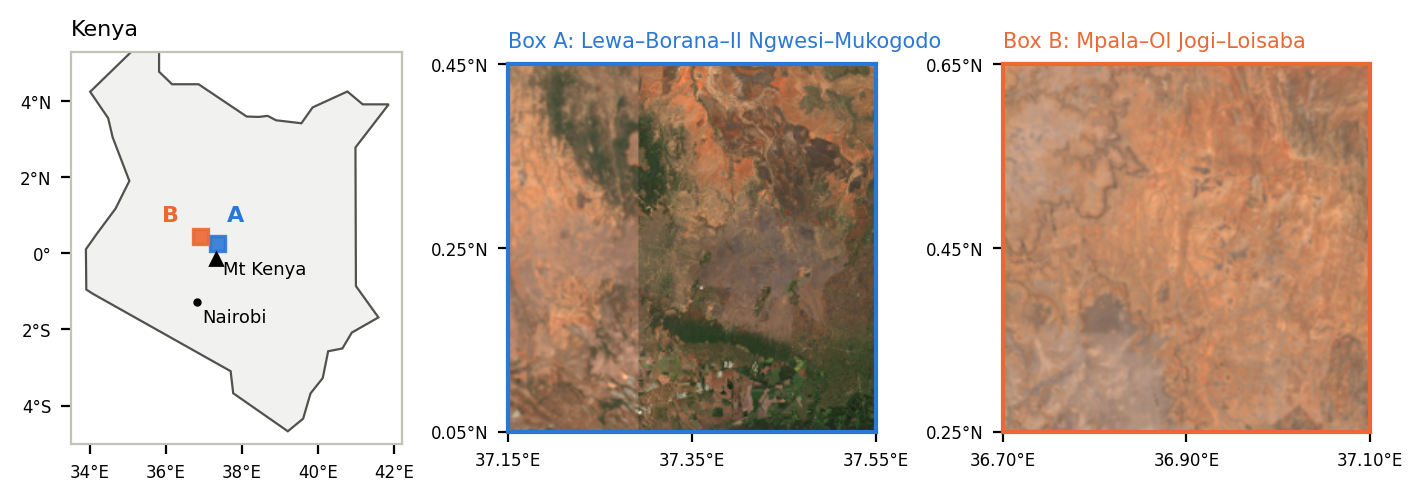
\includegraphics[width=\textwidth]{fig_map.png}
\caption{Where. Left: Kenya with the two $45$\,km boxes; Box A spans $37.15$--$37.55^\circ$E, $0.05$--$0.45^\circ$N, Box B $36.70$--$37.10^\circ$E, $0.25$--$0.65^\circ$N. Centre and right: Sentinel-2 true colour of each box in the 2023 dry season; dark green is forest and riverine woodland, pale is open rangeland. Contains modified Copernicus Sentinel data (2023).}
\label{fig:map}
\end{figure*}

\begin{table}[t]\centering\caption{Skill on held-out years 2019--25, $1-\mathrm{CRPS}/\mathrm{CRPS}_{\mathrm{M0}}$, one step (16 days) and three months along the observed weather, on Box A and on Box B, the unseen landscape. M2 and M3 are means of five fits. RESTREND gives season-end values only.}\label{tab:onestep}\footnotesize\setlength{\tabcolsep}{3pt}
\begin{tabular}{lcccc}\toprule
 & \multicolumn{2}{c}{Box A} & \multicolumn{2}{c}{Box B}\\
Model & 16 days & 3 months & 16 days & 3 months\\\midrule
M0 history only & 0.000 & 0.000 & 0.000 & 0.000\\
RESTREND & -- & 0.170 & -- & 0.190\\
M1 linear & 0.013 & 0.107 & 0.040 & 0.099\\
M2 learned & 0.092 & 0.241 & 0.075 & 0.177\\
M3 with topography & 0.099 & 0.254 & 0.083 & 0.204\\
M4 ensemble & \textbf{0.111} & \textbf{0.273} & \textbf{0.131} & \textbf{0.274}\\
\bottomrule\end{tabular}\end{table}

\begin{figure}[t]
\centering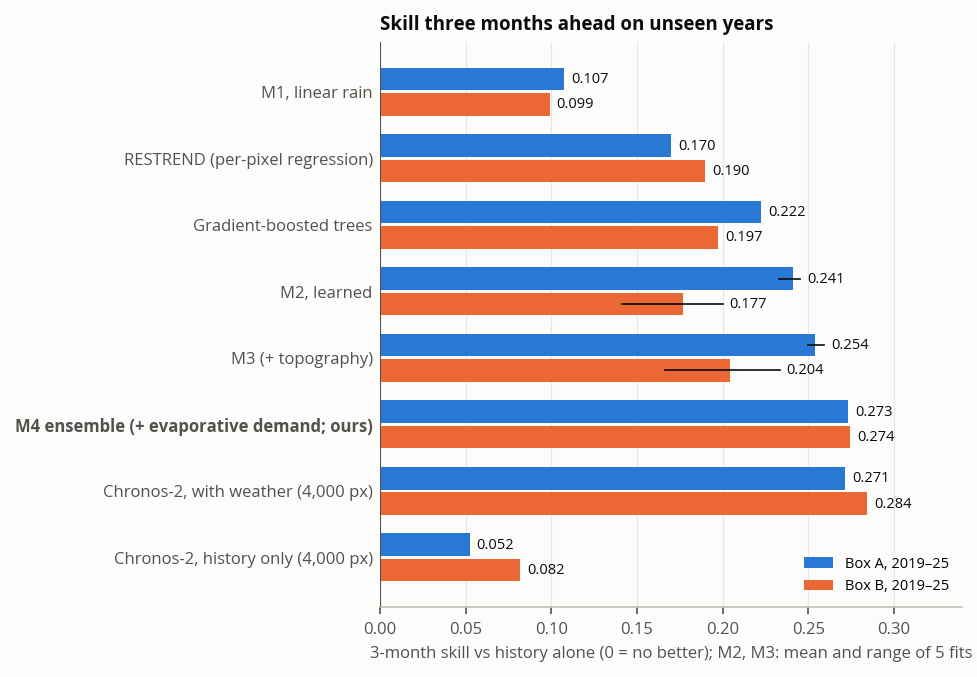
\includegraphics[width=\columnwidth]{candidates/fig_suite_skill.png}
\caption{Three-month skill on unseen years against history alone, given the weather that fell; no model uses a weather forecast. M2 and M3 show the mean and range of five fits. Chronos-2 \textbf{add Chronos-2 citation} is a pretrained forecaster, scored zero-shot on 4,000 sampled pixels, with and without the weather.}
\label{fig:response}
\end{figure}

\begin{table*}[t]\centering\caption{Pre-registered tests of $\Delta$ for the M4 ensemble, written before running; primary G1 on Box A. Held-out rainy-season starts 2019--25 whose two-step outcome does not span a MODIS gap. Gaps are the real response of the most minus the least $\Delta$ third (NDVI per $100$\,mm), given starting greenness. Brackets are $95\%$ bootstrap intervals over test years.}\label{tab:greekstests}\small
\begin{tabular}{lcc}\toprule
Test & Box A & Box B\\\midrule
G1 (primary), within pixel & $+.060$ $[+.027, +.085]$ pass & $+.018$ $[-.046, +.083]$ fail\\
G1, also given evaporative demand & $+.046$ $[+.015, +.065]$ pass & $-.027$ $[-.107, +.028]$ fail\\
G2, across pixels & $+.078$ $[+.054, +.105]$ pass & $+.021$ $[-.037, +.082]$ fail\\\bottomrule
\end{tabular}\end{table*}

\paragraph{Fitting} We use full-batch Adam \citep{kingma2015} at a learning rate of $3\times10^{-3}$ for up to 2000 steps, keeping the parameters with the best 2018 log-likelihood; each step uses all $25\,600$ pixels and the $\sim340$ training-year transitions. Each M4 fit has 1,002 parameters, and the ensemble is the equal-weight mixture of five fits from different seeds. One fit takes about $2.5$ minutes on one H100 and $80$ on a laptop CPU, and GPU and CPU fits agree to about $0.005$ in skill. Jacobian-vector products of the mean rollout, computed in JAX \citep{jax2018}, agree with finite differences to $3\times10^{-4}$, against a $\Delta$ of order $10^{-2}$. Code and the run directory behind every number are in the supplementary repository.
\bibliography{references}
\end{document}
